\documentclass[spanish,notitlepage,letterpaper, 12pt]{article} 
\usepackage[spanish]{babel} 
\usepackage{amsmath}
\usepackage{amsfonts}
\usepackage{amssymb}
\usepackage{graphicx}
\usepackage{geometry}      
\geometry{letterpaper}                  
\usepackage{epstopdf}
\usepackage{fancyhdr} % Paquete para encabezados y pies de pag
\usepackage{color}
\usepackage{placeins}
\usepackage{csquotes}
\usepackage{textcomp}
\usepackage{gensymb} 

\pagestyle{fancy} 
\chead{\bfseries Informe 6 - Grupo C1B. Subgrupo 2} 
\rhead{22 de Junio de 2023}
\cfoot{Universidad Industrial de Santander} 
\rfoot{\thepage} 

\voffset = -0.25in 
\textheight = 8.0in 
\textwidth = 6.5in
\oddsidemargin = 0.in
\headheight = 20pt 
\headwidth = 6.5in
\renewcommand{\headrulewidth}{0.5pt}
\renewcommand{\footrulewidth}{0,5pt}
\begin{document}
\begin{titlepage}
    \begin{center}
        
\includegraphics[width=0.4\textwidth]{../general-images/uis-logo.png}
        
        \vspace{0.5cm}
        \LARGE
        \textbf{Estudio del comportamiento del circuito RLC y el fenómeno de resonancia}
        
        \vspace{0.5cm}
        \large
        Informe 4
        
        \vfill
        
        \textbf{Daniel Esteban Vargas Reyes.} Estudiante - Geología\\
        \textbf{Nicolás Andrés Ramírez Calderón.} Estudiante - Ingeniería de Sistemas\\ 
        \textbf{Rodolfo Valentín Muñoz Vega.} Estudiante - Ingeniería Química\\

        \vspace{1.0cm}
        Presentado a la docente:
        
        \textbf{Zayda Paola Reyes Quijano}
        
        \vfill
        
        Escuela de Física - Física III\\
        Universidad Industrial de Santander\\
        Bucaramanga, Santander, Colombia\\
        20 de Mayo de 2023        
    \end{center}
\end{titlepage}

\tableofcontents

\newpage

\section{Resumen}
En el día a día es común manipular tecnologías de ultrasonido, infrarrojo y microondas
(controles de TV, alarmas para autos, los teléfonos celulares y hornos de cocina); no
obstante, no siempre distinguimos con claridad los medios de propagación y el
funcionamiento de estas tecnologías. Las ondas elásticas requieren un medio material
como soporte a su transmisión. Tal sucede con las ondas sonoras, ondas en cuerdas,
membranas, etc. En cambio, las ondas electromagnéticas no requieren de un medio
material para su propagación. En este proyecto, las microondas se presentan como un
fenómeno susceptible de mostrar dispersión, polarización, absorción, etc., al igual que
ocurre para la luz visible.
\section{Introducción}
En el presente proyecto, se estudió el fenómeno de polarización y absorción de las
microondas con el fin de comprender la propagación y distribución en el medio cercano al
emisor.
\subsection{Marco teórico} \label{I.MT}
Las microondas están situadas entre los rayos infrarrojos (cuya frecuencia es mayor) y
las ondas de radio convencionales. Su longitud de onda va aproximadamente desde $1
mm$ hasta $30 cm$. Las microondas se generan con tubos de electrones especiales como el
klistrón o el magnetrón, que incorporan resonadores para controlar la frecuencia, o con
osciladores o dispositivos de estado sólido especiales. En este proyecto, se empleó
como detector de campo eléctrico una sonda $E$, con la que se mide la componente del
campo eléctrico paralela a la sonda. La señal de salida de la sonda es proporcional al
cuadrado de la intensidad del campo y con ello a la intensidad de las ondas.\par
\begin{equation}
    E(\theta)=E_0\cos{\theta}
\end{equation}
Las microondas pueden polarizarse como las ondas de luz. Si el campo eléctrico oscila en
un plano fijo, esto se llama polarización lineal. Si una onda linealmente polarizada con una
amplitud de campo eléctrico $E_0$ incide en un polarizador que se gira respecto a la dirección
de polarización de la onda por un ángulo $\theta$, la componente del campo pasa al polarizador. Por consiguiente, la intensidad de la onda es detrás de polarizador.\par
\begin{equation}
    I(\theta)=I_0\cos^2(\theta)
\end{equation}
Existe una marcada diferencia entre la generación de microondas y las ondas de luz. Las
microondas se generan en una guía de onda y se emiten en el espacio libre vía una
antena extensa. A una distancia suficientemente grande, la antena puede considerarse
como una fuente puntual. A esta distancia los campos eléctrico y magnético de las
microondas oscilan perpendicularmente uno del otro y en la dirección de la propagación
(campo lejano) \cite{serway_jewett_2017}. Ambos campos disminuyen de manera inversamente proporcional a la
distancia y su razón es constante como indica la ecuación \eqref{eq:sim-e-b}.
\begin{equation}\label{eq:sim-e-b}
    E_0\sim B_0\sim\frac{1}{r}
\end{equation}
Mientras que a distancias por debajo del límite se maneja la ecuación \eqref{eq:d-lam}.
\begin{equation}\label{eq:d-lam}
    r_{D}=2\frac{D^2}{\lambda}
\end{equation}
Para la ecuación \eqref{eq:d-lam}, $D$ representa la dimensión transversal mayor de la antena, $\lambda$ es la longitud de onda de la distribución del campo de la onda\par
\bigskip
Sólo en ondas radiadas perpendicularmente a la antena, la dirección de propagación y el
campo eléctrico y magnético son perpendiculares unos a otros. Cuando las microondas
atraviesan una superficie, parte de la potencia de microondas es absorbida en el medio,
haciéndolo un sistema subamortiguado. La proporción absorbida depende del espesor del
medio y la estructura molecular.\par
\subsubsection{Absorción}
Cuando una onda electromagnética se propaga a través de la atmósfera terrestre, se
transfiere energía de la onda a los átomos y moléculas que componen la atmósfera. La
absorción de onda por la atmósfera es análoga a una pérdida de potencia $I^2R$. Una vez
absorbida, la energía se pierde (en otras formas) y causa una atenuación en las
intensidades de voltaje y campo magnético, así como una reducción correspondiente de
densidad de potencia.
\section{Metodología}
\subsection{Materiales}
\begin{itemize}
    \item Oscilador Gunn.
    \item Antena de bocina grande.
    \item Fuente de alimentación Gunn.
    \item Sonda de campo $E$.
    \item Accesorios de microondas.
    \item Voltímetro.
    \item Bases cilíndricas.
    \item Cables.
\end{itemize}
\subsection{Fase 1}
En esta primera fase, se verificó la distribución del potencial eléctrico delante
del emisor del microondas (antena tipo bocina). Para esto, fue necesario realizar el
montaje pertinente (Fig. \ref{fig:montaje1}). Primero, se deberá contó con una plantilla que contenga un eje de
coordenadas. Luego, se ubicó la antena en la coordenada $(0,0)$. Segundo, se situó la sonda de campo eléctrico en el eje central o longitudinal $(X)$, posteriormente, se
varió la posición de la sonda en diferentes coordenadas sobre el eje central (designadas
por el docente) para finalmente medir y tabular los diferentes valores de tensión con el
voltímetro en las diferentes coordenadas establecidas anteriormente.\par
\begin{figure}[!ht]
    \centering
    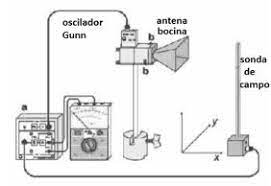
\includegraphics[width=10.0cm]{images/montaje1.jpeg}
    \label{fig:montaje1}
    \caption{\textit{Montaje experimental, distribución del campo eléctrico delante de la bocina.}}
\end{figure}
De forma similar, se procedió a medir el campo eléctrico de forma transversal, moviendo
la sonda en diferentes coordenadas del eje $(Y)$. Por último, se realizó el análisis
gráfico de la distribución del campo eléctrico.
\subsection{Fase 2}
En esta fase se estudió la relación entre la intensidad de la onda y el ángulo
del polarizador sobre microondas, frecuencia $9.4 GHz$. Para ello, fue necesario realizar el
montaje (Fig. \ref{fig:montaje2}) empleando una rejilla de polarización compuesta con tiras delgadas
de metal, donde el campo eléctrico se forma perpendicularmente a las tiras. Primero, se
situó la bocina en las coordenadas $(0,0)$ y la sonda se ubicó a una distancia
longitudinal $X$ designada por el docente. En esta ubicación se registró el valor de la
tensión ($U_0$) y luego se ubicó la rejilla de polarización en la parte media entre la antena y
la sonda $E$.\par
\begin{figure}[!ht]
    \centering
    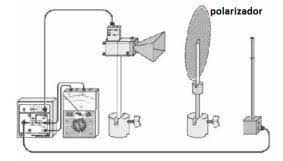
\includegraphics[width=10.0cm]{images/montaje2.jpeg}
    \label{fig:montaje2}
    \caption{\textit{Polarización de microondas.}}
\end{figure}
Segundo, con la ayuda de un voltímetro se registraron los valores de voltaje en cada una de las
posiciones que el polarizador trae entre $0$° y $360$°. Tercero, se repitió procedimiento anterior
varias veces y se promediaron los valores de voltaje. se registraron los datos, se normalizaron
los valores del voltaje promedio, $\frac{U_{prom}}{max(U_{prom})}$
. Posteriormente, se cambió la antena
de posición conservándola en coordenada $(0,0)$ y repitiendo el procedimiento anterior
registrando los datos.
\subsection{Fase 3}
En esta fase se analizó el fenómeno de absorción en diferentes materiales a
partir de la intensidad incidente y transmitida. Fue necesario realizar un montaje similar
al de la fase uno: antena en coordenadas $(0,0)$ y la sonda en una posición longitudinal $x$
(determinada por el docente). En esta posición se midió el valor de la tensión ($U_0$).\par
\newpage
\begin{figure}[!ht]
    \centering
    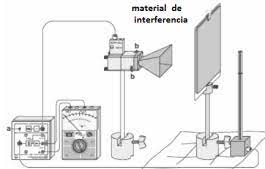
\includegraphics[width=10.0cm]{images/montaje3.jpeg}
    \label{fig:montaje3}
    \caption{\textit{Arreglo experimental para medir la absorción de microondas.}}
\end{figure}
Segundo, se introdujeron diferentes materiales en medio de la bocina y la sonda,
tabulando los datos para cada uno de los diferentes materiales suministrados
por el docente. Por último, se calculó el coeficiente de absorción de la siguiente
ecuación \eqref{eq:abs-per}.\par
\begin{equation}\label{eq:abs-per}
    \propto\ (\%)=(\frac{U_0-U}{U_0})100
\end{equation}
\section{Tratamiento de datos} \label{TD}
\section{Análisis de resultados}
\section{Conclusiones}
\section{Referencias} 
\bibliographystyle{unsrt}
\bibliography{../general-references/references}
\end{document}
